\documentclass[10pt, a4paper]{article}
\usepackage{geometry}
\usepackage{graphicx}

 \geometry{
 a4paper,
 total={170mm,257mm},
 left=20mm,
 top=20mm,
 }
 \usepackage{hyperref}
\hypersetup{
    colorlinks=true,
    linkcolor=black,
    filecolor=magenta,      
    urlcolor=cyan,
}
\title{Guida porting RTEMS su Raspberry Pi}
\author{Clark Ezpeleta}
\usepackage{parskip}
\usepackage{listings}

\begin{document}
\pagenumbering{gobble}
\maketitle
\newpage
\tableofcontents
\newpage
\pagenumbering{arabic}
\begin{flushleft}
\section{Introduzione}
Guida per l'installazione di RTEMS RSB e della tool-suite per l' utilizzo del kernel di RTEMS su architetture ARM, con target le BSP di Raspberry Pi 1 e Raspberry Pi 2, quest'ultima è compatibile con la Raspberry pi 3.

Il RSB (RTEMS Source Builder) è un tool per buildare i pacchetti dai file sorgenti. Viene usato in RTEMS per buildare i suoi compilatori e OS.

La BSP (Board Support Package) è il codice di supporto per una specifica scheda, esso contiene librerie di RTEMS utili per l'utilizzo della scheda.

Poichè RTEMS è un progetto open source ancora in sviluppo, al momento stanno sviluppando la v6, ma non è ancora stabile, per questo motivo in questa guida si installerà la v5.1 che è la versione stabile più recente.

Durante questa guida viene usato il sistema operativo Ubuntu LTS 20.04.

\newpage
\section{Configurazione iniziale del sistema}
Prima di iniziare l'installazione di RTEMS RSB e tool-suite bisogna configurare l'ambiente di sviluppo.

Procediamo con l'installazione dei seguenti pacchetti:
\begin{itemize}
\item  build-essential : 
\begin{lstlisting}[language=bash] 
$ sudo apt-get install build-essential
\end{lstlisting}
\item git:
\begin{lstlisting}[language=bash] 
$ sudo apt-get install git
\end{lstlisting}
\item python-dev:
\begin{lstlisting}[language=bash] 
 $ sudo apt-get install python-dev
 \end{lstlisting}
\end{itemize}

A questo punto definiamo la struttura delle cartelle in cui verranno installati i componenti di RTEMS.

\begin{itemize}
\item \$HOME/rtems-dev  : base directory
\item \$HOME/rtems-dev : base directory dove vengono clonati da git la tool-suite e la RSB di RTEMS
\item \$HOME/rtems-dev/src/rsb : RTEMS source builder
\item \$HOME/rtems-dev/src/rtems : RTEMS tool-suite
\item \$HOME/rtems-dev/rtems/ : dove verrà installata la RTEMS tool-suite
\item \$HOME/rtems-dev/build : dove verranno installate le BSP di Rpi1 e Rpi2
\end{itemize}
\newpage
\section{Installazione RTEMS}

Dopo aver preparato l'ambiente di sviluppo, possiamo procedere con l'installazione di RTEMS:
\begin{itemize}

\item Cloniamo i repository della RTEMS RSB e della tool-suite : 
\begin{lstlisting}[language=bash] 
$ mkdir - p $HOME/rtems-dev/src
$ cd $HOME/rtems-dev/src
$ git clone -b 5.1 git://git.rtems.org/rtems-source-builder.git rsb
$ git clone -b 5.1 git://git.rtems.org/rtems.git
\end{lstlisting}

\item Eseguiamo la build e l'installazione della tool suite utilizzando la RSB :
\begin{lstlisting}[language=bash] 
$ cd $HOME/rtems-dev/src/rsb/rtems
$ ../source-builder/sb-set-builder --prefix= $HOME/quick-start/rtems/5 5/rtems-arm
\end{lstlisting}

\item Dopo aver completato l'installazione possiamo controllare che il C cross compiler di RTEMS sia stato installato correttamente utilizzando il seguente comando: 
\begin{lstlisting}[language=bash] 
$ $HOME/rtems-dev/rtems/5/bin/arm-rtems5-gcc --version
\end{lstlisting}	
e si ha come risultato:
\begin{figure}[h!]
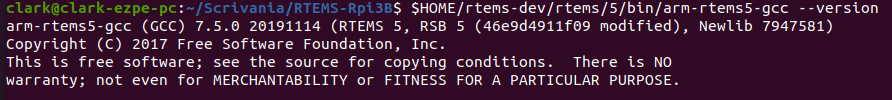
\includegraphics[width=\linewidth]{rtems-gcc-version.png}
\end{figure}

\item Inseriamo nelle variabili di ambiente i comandi della toolchain e procediamo con il bootstrap : 
\begin{lstlisting}[language=bash] 
$ export PATH=$HOME/rtems-dev/rtems/5/bin:"$PATH" (3.1)
$ cd $HOME/rtems-dev/src/rtems
$ ./rtems-bootstrap
\end{lstlisting}	
	
\item Adesso possiamo configurare ed installare le BSP che ci servono: 
\begin{lstlisting}[language=bash] 
$ mkdir -p $HOME/rtems-dev/build
$ cd $HOME/rtems-dev/build
$ $HOME/rtems-dev/src/rtems/configure \
        --prefix=$HOME/quick-start/rtems/5 \
	--target=arm-rtems5 \
	--enable-rtemsbsp="raspberrypi raspberrypi2"\
	--enable-tests=samples --enable-networking --enable-posix
$ make
$ make install	
\end{lstlisting}
		
\end{itemize}

Svolti tutti i passaggi precedenti abbiamo come risultato RTEMS installato sul computer host.
\newpage
\section{Prova sample test RTEMS}

Installando le BSP, RTEMS ci fornisce dei sample test .exe da cui possiamo generare i file .img e utilizzarli per testare il funzionamento della raspberry pi

I sample test sono in : 
\begin{itemize}
\item  rpi 1:
\begin{lstlisting}[language=bash] 
$ $HOME/rtems-dev/build/arm-rtems5/c/raspberrypi1/testsuites/samples
\end{lstlisting}
\item  rpi 2 e 3:
\begin{lstlisting}[language=bash] 
$ $HOME/rtems-dev/build/arm-rtems5/c/raspberrypi2/testsuites/samples
\end{lstlisting}
\end{itemize}

In questa guida utilizziamo il sample 'ticker.exe', ma i passaggi che verranno illustrati valgono anche per gli altri sample presenti in cartella.
Per poter utilizzare il sample test dobbiamo fare 2 passaggi:
\begin{itemize}
\item Creazione kernel file .img:

assicurarsi di avere come variabile di ambiente i comandi della tool-suite:
\begin{lstlisting}[language=bash] 
$ echo $PATH
\end{lstlisting}
se non è presente  '\$HOME/rtems-dev/rtems/5/bin' allora bisogna inserirla (vedi comando 3.1).

posizionarsi nella cartella dove vogliamo che venga creato il file .img:
\begin{lstlisting}[language=bash] 
$ cd $HOME/rtems-dev/rtems 
\end{lstlisting}		

generare il file .img:

Per Rpi1: 
\begin{lstlisting}[language=bash] 
$ arm-rtems5-objcopy -Obinary $HOME/rtems-dev/build/arm-rtems5/c/raspberrypi1/ 
testsuites/samples/ticker.exe ticker.img
\end{lstlisting}
Per Rpi2 e Rpi3: 
\begin{lstlisting}[language=bash ] 
$ arm-rtems5-objcopy -Obinary $HOME/rtems-dev/build/arm-rtems5/c/raspberrypi2/
testsuites/samples/ticker.exe ticker.img
\end{lstlisting}

\item Configurare la SD card:
copiamo nella scheda sd il firmware di Rpi (v4.19.11.3) compatibile con RTEMS. 
Il firmware puo' essere scaricato da questo link:  \\
\small\url{https://github.com/raspberrypi/firmware/tree/5574077183389cd4c65077ba18b59144ed6ccd6d/boot}
Eliminiamo tutti i file kernel*.img, questi verranno sostituiti dal file 
kernel che abbiamo generato precedentemente.
Copiamo nella sd il file ticker.img creato precendetemente.
Creiamo nella sd il file config.txt che contiene il seguente testo:
\begin{lstlisting}[language=bash ] 
		enable_uart=1
		kernel_address=0x200000
 		kernel=ticker.img 
\end{lstlisting}
Nel campo kernel mettiamo il nome del kernel file che vogliamo che rpi esegua.
\end{itemize}
	
\newpage
 	 
A questo punto siamo pronti con il test.

Per poter vedere la log della UART dobbiamo installare minicom:
\begin{lstlisting}[language=bash] 
$ sudo apt-get install minicom
\end{lstlisting}

Colleghiamo il convertitore UART alla Rpi :
\begin{figure}[h!]
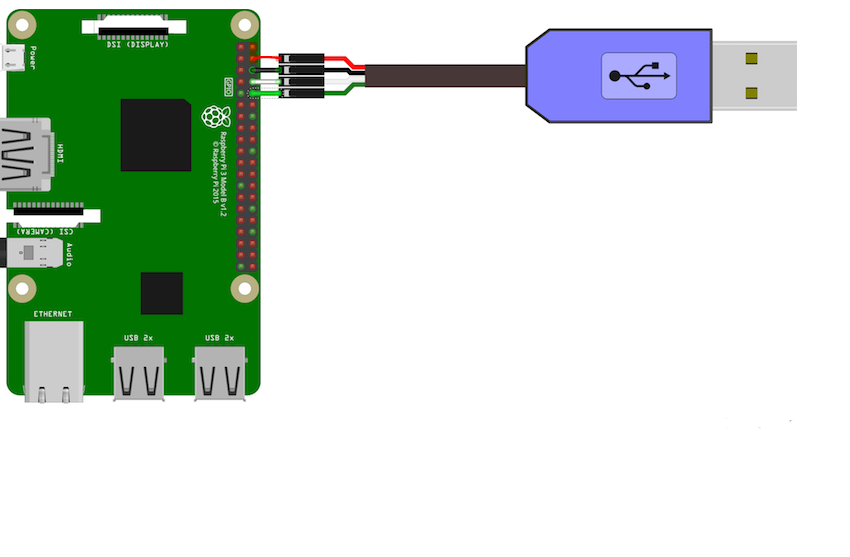
\includegraphics[width=\linewidth]{rpi-uart-usb.png}
\end{figure}
\\
dove i GPIO pin sono :
\begin{figure}[h!]
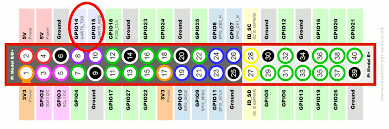
\includegraphics[width=\linewidth]{rpi-gpio.png}
\end{figure}

\newpage
Colleghiamo la chiaveta USB al computer ed eseguiamo il comando per vedere la log della UART :
\begin{lstlisting}[language=bash] 
$ sudo minicom -b 115200 -D /dev/serial/
by-id/<indirizzo periferica utilizzata per UART di solito un USB TTL>
\end{lstlisting}

il risultato dovrebbe essere simile a questo:
\begin{figure}[h!]
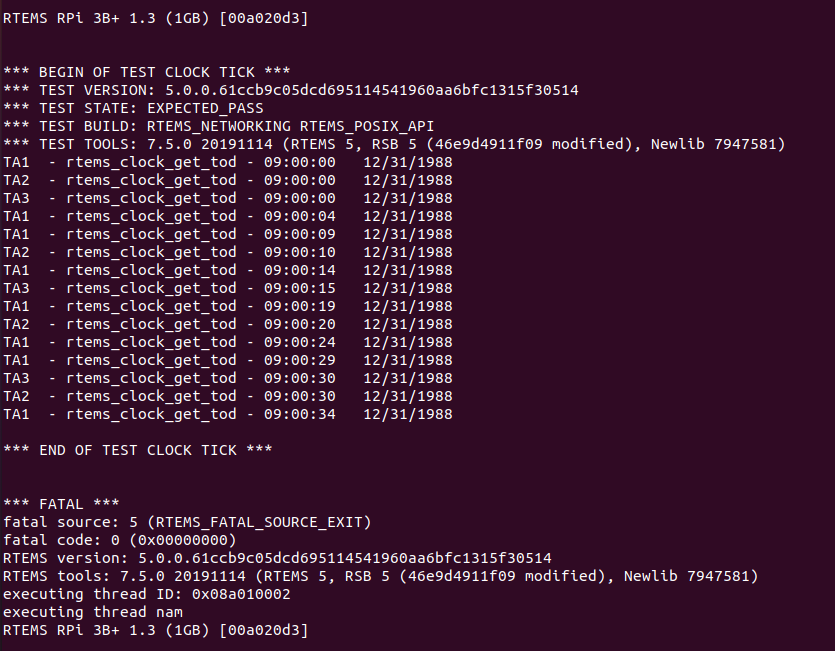
\includegraphics[width=\linewidth]{risultato-ticker.png}
\end{figure}

\newpage
\section{Configurazione Eclipse C/C++} 
Per creare i file sorgenti per programmi di RTEMS possiamo utilizzare l'IDE Eclipse C/C++ scaricabile da questo link :
\url{https://www.eclipse.org/downloads/packages/}


Una volta installato Eclipse C/C++ bisogna installare il plugin di RTEMS:
\begin{itemize}
\item Andiamo su Help> Install New Software
\item Aggiungiamo come Software site quello di RTEMS, quindi clicchiamo add e inseriamo il seguente url \url{ftp://ftp.rtems.org/pub/rtems/eclipse/updates}
\begin{figure}[h!]
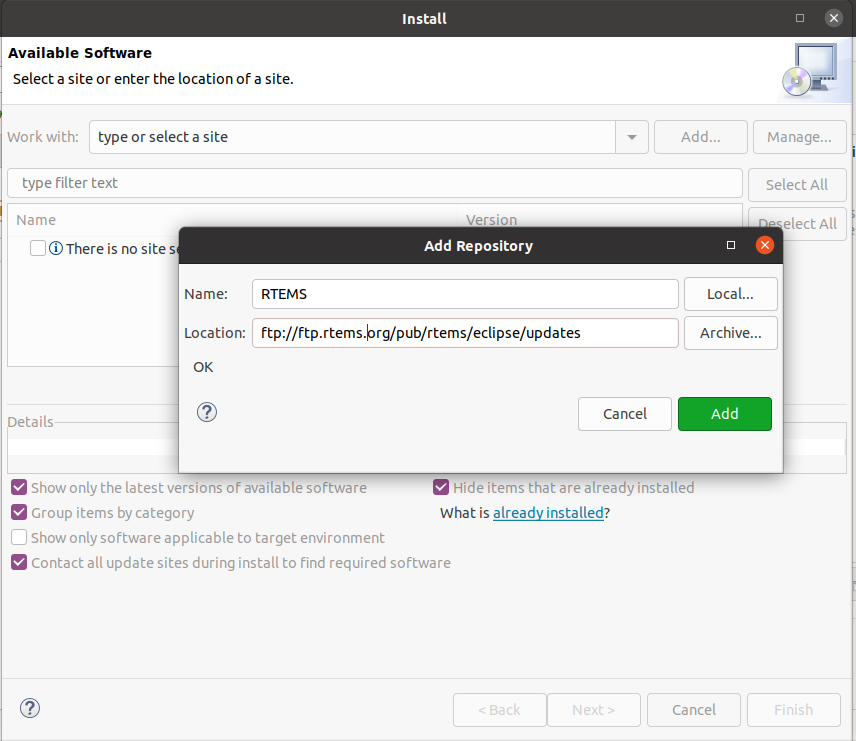
\includegraphics[width=\linewidth]{ftp-rtems-eclipse.png}
\end{figure}
\item Selezioniamo il plugin RTEMS CDT Support e installiamo
\end{itemize}

A questo punto abbiamo installato il plugin di RTEMS ed è pronto ad essere utilizzato.

\newpage

Quando creiamo un progetto RTEMS bisogna configurare la base e il BSP path di RTEMS in modo che si riesca ad utilizzare le librerie che ci servono:
\begin{itemize}
\item Window $\rightarrow$ Preferences $\rightarrow$ C/C++ $\rightarrow$ RTEMS
\item Base path : base path dell'installazione , nel nostro caso home/<username>/rtems-dev/rtems/5
\item BSP path : path dell'installazione della BSP, nel nostro caso home/<username>/rtems-dev/rtems/5/arm-rtems5/raspberrypi2 (o 1 se si utilizza Rpi1)
\end{itemize}

\begin{figure}[h!]
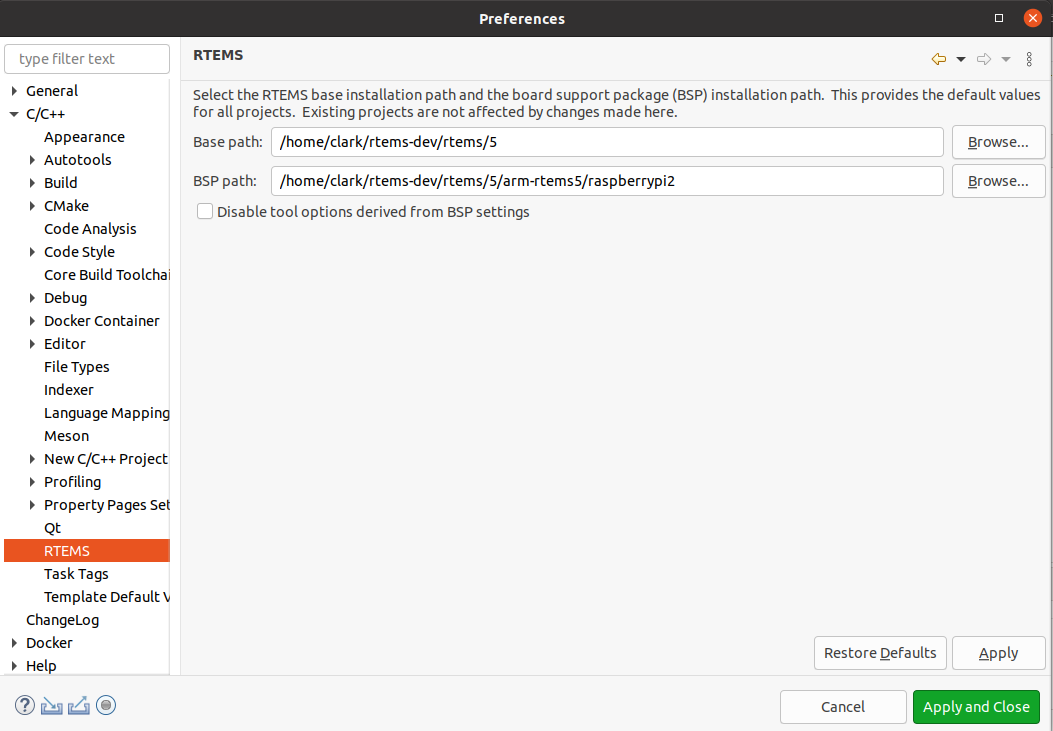
\includegraphics[width=\linewidth]{rtems-path-eclipse.png}
\end{figure}

\newpage

Abbiamo completato la configurazione del plugin di RTEMS su Eclipse C, adesso possiamo procedere alla creazione di un progetto RTEMS:
\begin{itemize}
\item New project$\rightarrow$ C Project
\item Selezionare il project type corretto: Others$\rightarrow$ RTEMS Executable
\item Selezionare la Toochain corretta : RTEMS Toolchain
\end{itemize}
\begin{figure}[h!]
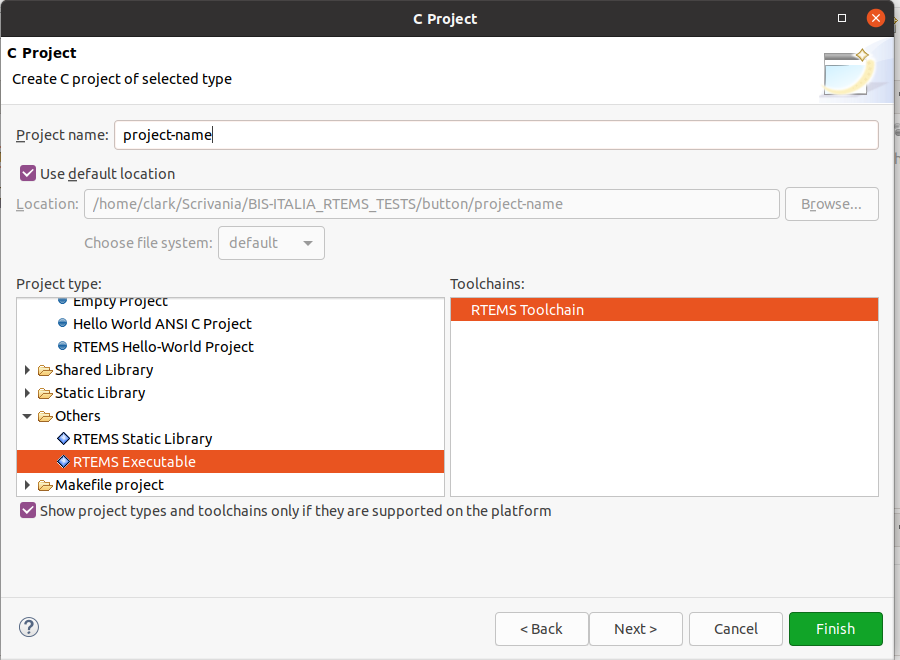
\includegraphics[width=\linewidth]{new-c-project.png}
\end{figure}
Possiamo controllare che il progetto è stato creato correttamente controllando le sue properties $\rightarrow$ C/C++ Build $\rightarrow$ RTEMS i path siano quelli corretti.

\newpage
\section{Prova con Eclipse C/C++}

Possiamo adesso fare un semplice programma di prova "hello world",
creiamo 2 file sorgenti:
- init.c : conterrà il task principale (Init) che è il task di "ingresso".
- system.c : conterrà il codice di configurazione di RTEMS.

in init.c inseriamo il seguente codice:
\begin{lstlisting}[language=c] 

/*
 * Hello world example
 */
#include <rtems.h>
#include <stdlib.h>
#include <stdio.h>
#include <bsp/mmu.h>

rtems_task Init(rtems_task_argument ignored) {
	printf("\n\n*** HELLO WORLD TEST ***\n");
	printf("Hello World\n");
	printf("*** END OF HELLO WORLD TEST ***\n");
	exit(0);
}


\end{lstlisting}
in system.c inseriamo il seguente codice :

\begin{lstlisting}[language=c] 

/*
 * Simple RTEMS configuration
 */

#define CONFIGURE_APPLICATION_DOES_NOT_NEED_CLOCK_DRIVER
#define CONFIGURE_APPLICATION_NEEDS_SIMPLE_CONSOLE_DRIVER

#define CONFIGURE_UNLIMITED_OBJECTS
#define CONFIGURE_UNIFIED_WORK_AREAS

#define CONFIGURE_RTEMS_INIT_TASKS_TABLE

#define CONFIGURE_INIT

#include <rtems/confdefs.h>

\end{lstlisting}

per una migliore comprensione del codice si rimanda ai seguenti link:
\begin{itemize}
\item per le api: \\ \url{https://devel.rtems.org/browser/rtems/bsps/arm/raspberrypi}
\item per la configurazione di rtems su codice (system.c):\\  \url{https://ftp.rtems.org/pub/rtems/people/joel/docs-eng/c-user/configuring_a_system.html}
\end{itemize}

A questo punto possiamo buildare il programma, e nella cartella del progetto troveremo la cartella 'RTEMS Executable Configuration' che contiene il file .exe che utilizzeremo per creare il file .img da mettere nella scheda SD.
I passaggi per la creazione del file .img sono sopracitati.

\newpage
\section{Creazione file kernel senza IDE}
Se si vuole creare il file .img partendo dai file sorgente allora dobbiamo usare i seguenti comandi nel terminale:
\begin{itemize}
\item ci posizioniamo nella cartella dove ci sono i file sorgenti.
\item eseguiamo i comandi del cross compiler di RTEMS su tutti i file .c: 
\begin{lstlisting}[language= bash] 
 $ $HOME/rtems-dev/rtems/5/bin/arm-rtems5-gcc -B \
   $HOME/rtems-dev/rtems/5/arm-rtems5/raspberrypi2/lib/ \
   -specs bsp_specs -qrtems -ffunction-sections -fdata-sections \
   -march=armv7-a -mthumb -mfpu=neon -mfloat-abi=hard -mtune=cortex-a7 \
   -Os -g -Wall -c -fmessage-length=0 -pipe -MMD -MP -MF"init.d" \
   -MT"init.o" -o "init.o" "../init.c"
\end{lstlisting}
\item utilizziamo il linker per la creazione del file .exe :
\begin{lstlisting}[language= bash] 
$ $HOME/rtems-dev/rtems/5/bin/arm-rtems5-gcc -B \
  $HOME/rtems-dev/rtems/5/arm-rtems5/raspberrypi2/lib/ \
  -specs bsp_specs -qrtems -ffunction-sections -fdata-sections \
  -march=armv7-a -mthumb -mfpu=neon -mfloat-abi=hard -mtune=cortex-a7 \
  -Wl,--gc-sections -o "hello-rpi.exe"  ./init.o ./system.o    
\end{lstlisting}

\end{itemize}
\item a questo punto possiamo creare il file .img e copiarlo sulla scheda sd e fare i passaggi già esposti precedentemente.

\newpage
\section{Troubleshooting}

\newpage
\section{Sitografia}
\begin{itemize}
\item Documentazione RTMES :\\ \url{https://docs.rtems.org/branches/master/user/index.html}
\item Guida RTEMS di Giorgio :\\ \url{https://gist.github.com/giorgiobasile/1c1930a8a3ff8e36061cd7f4ef83da95}
\item Sito spiegazione porting RTEMS (Alan Tech):\\ \url{http://alanstechnotes.blogspot.com/2013/03/rtems-on-raspberry-pi.html} 
\item Documentazione API RTEMS:\\ \url{https://docs.rtems.org/branches/master/c-user/index.html}
\end{itemize}

\end{flushleft}


\end{document}
